%----------------------------------------------------------------------------
\chapter{Bevezető} 
%----------------------------------------------------------------------------

Egyetemi gyakorlatok során a hallgatók egy előre összeállított környezetben (például virtuális
gépeken) dolgoznak, melyet a tárgy oktatói készítenek el. Adott tanóra kezdése előtt 
ez azzal a feladattal jár, hogy bizonyos fájlokat kell a megfelelő gépekre eljuttatni. Ezeknek a gyakran nagy méretű fájloknak a több helyre történő másolása ``kézzel'', vagyis egy adathordozóval körbejárva a termet igen időigényes és körülményes lenne, ezért használnak az oktatók egy Chaincast\cite{kiraly2011chaincast} alapú programot a folyamat felgyorsítására. 

%----------------------------------------------------------------------------
\section{Problémafelvetés}
%----------------------------------------------------------------------------

Az előbb ismertetett terítési megoldás használatával kapcsolatban több probléma is felmerül:

\begin{itemize}
  \item Ha adatküldés közben a lánc bárhol megszakad, akkor az egész folyamatot kezdhetjük elölről, ami komoly skálázhatósági problémákhoz vezet, mivel minél több gépet kapcsolunk be a küldési láncba, annál valószínűbb, hogy a terítés meg fog szakadni egy hiba miatt.
   \item A program konfigurálása körülményes: ha például egy újonnan indult tanórára készítenénk fel a termet, ahol nem az összes gépre vagy az első három sorban levő levőkre szeretnénk teríteni, akkor a programban erre új küldési láncot kell definiálnunk.
   \item A terítést a tárgyak oktatói végzik, akik nem rendszergazdák: egyes fellépő problémákat nem feltétlen tudnak maguktól elhárítani, akár nem is rendelkeznek megfelelő jogosultságokkal. Ebbe beletartozik a használt alkalmazásnak a megfelelő beállítása, illetve a terítés során fellépő hibák kijavítása.
\end{itemize}

%----------------------------------------------------------------------------
\section{Célkitűzés}
%----------------------------------------------------------------------------

Célul tűzöm ki, hogy a most használt, Chaincast alapú fájlterítő megoldás kiváltására egy olyan alternatívát hozzak létre, ami a következő tulajdonságokkal rendelkezik az előbb ismertetett problémákat kijavítva:

\begin{itemize}
  \item Robusztus, skálázódó fájlterítés, amit úgy érek el, hogy a fájlok szétosztásában a célgépek is aktívan részt vesznek, úgynevezett Peer-to-Peer\cite{p2pdef} hálózatot alkotva.
  \item Egyszerű konfiguráció és használat, mivel egy, a laborunkat ábrázoló modell elkészítése és adatainak kitöltése után csak egy konkrét célállapotot kell megadni a terítési műveletek végrehajtásához.
  \item Virtuális gépek létrehozásának támogatása Vagrant\cite{vagrant} segítségével, ami automatizáltan képes egy konfigurációs fájl alapján VM-eket létrehozni és a felhasználó igényeinek megfelelően beállítani.
\end{itemize}

%----------------------------------------------------------------------------
\section{Kontribúció}
%----------------------------------------------------------------------------
Dolgozatomban bemutatok egy módszert modellvezérelt fájlterítésre, majd erre adok egy P2P alapú, Torrent protokollt használó implementációt. A kész szoftver specifikációnak megfelelő működését elenőrzöm, és mérésekkel elemzem annak különbőző teljesítménymutatóit a most használt megoldáséival összehasonlítva. Végül felvázolok pár lehetőséget a készített alkalmazás funkcióniak lehetséges bővítésére.

%----------------------------------------------------------------------------
\section{Hozzáadott érték}
%----------------------------------------------------------------------------
A programom az alábbiakkal fog többet nyújtani az előző megoldással szemben:

\begin{itemize}
  \item A fájlterítés olyan esetekben is sikerrel fog járni ahol régen nem. Például, ha a letöltés közben megszakad a kapcsolat az egyik célgéppel: itt régen a teljes folyamat megszakadt volna, most viszont sikerülni fog, sőt a kieső gép helyreállításakor arra is fel fognak végül kerülni a terítendő fájlok.
  \item Jól dokumentált API-val rendelkező Java nyelven írodott alkalmazás a mostani Bash szkripthez képest, ami jelentősen könnyít a karbantarthatóságon, ill. továbbfejleszthetőségen.
  \item Rugalmas: a modellalapú vezérlésnek köszönhetően nem csak abban az egy laborban vehető igénybe, ahol most a Chaincast van használva, hanem akár teljesen más laborokban is.
\end{itemize}

%----------------------------------------------------------------------------
\section{Korábbi munkák}
%----------------------------------------------------------------------------
Mielőtt nekiállunk a feladatot megoldani, érdemes lehet utánajárni, hogy milyen megoldások léteznek már fájlterítésre, ezek közül mutatok be itt röviden hármat:

\begin{itemize}
  \item \textbf{Chaincast}: A laborban most alkalmazott terítési módszer, egy láncot épít a terítésben résztvevő gépekből, ahol minden gép a kapott adatokat lementi és a láncban következőnek továbbítja. Működését \aref{fig:chaincast}-es ábra szemléltet. Az ábrán 3 gépet látunk egy 4 csomagra felvágott állomány terítése közben.
  \item \textbf{Fcast}\cite{gemmell2000fcast}: A sima IP Multicast üzenetküldés hiányosságait kijavítva ér el gyors és robusztus multiplexált adatátvitelt. Az IP Multicast protokoll használata során olyan üzeneteket küldünk, aminek nem egy konkrét címzettje van hanem egy címtartomány, így azokat a címtartományba eső összes aktív gép meg fogja kapni, és azok fogják eldönteni, hogy ``érdekli-e" őket a beérkezett üzenet. A protokoll nem biztosít semmilyen garanciát, hogy a küldött csomagok célba érnek, ezért az erre épülő adatátviteli módszerek gyakran úgy működnek, a végpontok ACK/NACK-ot (pozitív/negatív visszajelzést) küldenek a forrásnak az üzenetek érkezéséről, viszont ez könnyen túlterhelheti azt, vagy valamelyik előtte levő hálózati eszközt. Erre az ismert problémára ad megoldást az Fcast úgy, hogy a küldendő adatokat feldarabolja, és az utolsó darab küldése után újrakezdi a küldést, így ha valamelyik végpont nem kapott meg egyet, így azt pótolhatja. A szaknyelvben ezt az újraküldési technikát data carousel-nek, vagyis adat-körhintának hívják.
  \item \textbf{FastReplica}\cite{cherkasova2003fastreplica}:  Egy olyan fájlterítésre használt algoritmus, amit főleg tartalomszolgáltató hálózatokban(CDN) használnak. Működésének alapja, hogy a küldendő fájlnak különböző darabjait küldjük el a célcsomópontoknak, akik a kapott darabot tovább kell hogy küldjék az összes másik csomópontnak.
  \item \textbf{BitTorrent Sync}\cite{farina2014bittorrent}: Az ismert központosított felhő-alapú fájlszinkronizációs szolgáltatásokra(Dropbox, Google Drive \ldots) nyújt elosztott, Bittorrent alapú alternatívát. Tetszőleges számú gép között tud fájlokat szinkronizálni, az adatátvitel titkosított csatornán folyik és a lokális fájlok is opcionálisan titkosíthatóak. Új fájl hozzáadásánál az eredeti példányt tartalmazó gép seed, a szinkronizáció célgépei leecher szerepet fognak betölteni (a Bittorrent protokoll terminológiájával kapcsolatban lásd \aref{sect:p2p}-es fejezetet).
\end{itemize}

\begin{figure}[ht]
\centering
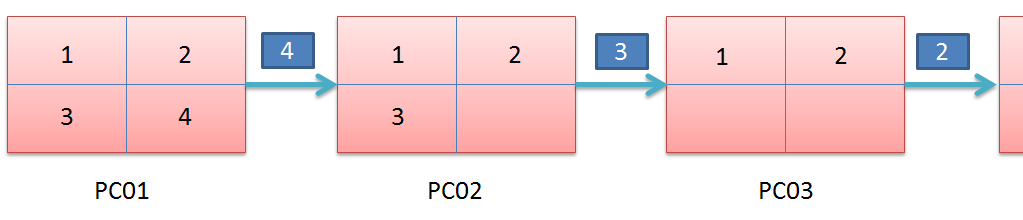
\includegraphics[width=140mm, keepaspectratio]{figures/chaincast.png}
\caption{Chaincast-os terítés működése - a legutóbb megkapott fájldarabot továbbküldjük a láncban következő gépnek}
\label{fig:chaincast}
\end{figure}

%----------------------------------------------------------------------------
\section{Dolgozat felépítése}
%----------------------------------------------------------------------------

Dolgozatom a következőképpen épül fel:
\Aref{chp:background}.~fejezetben bemutatom a munkám során használt fontosabb technológiákat és a megértéséhez szükséges háttérismereteket. \Aref{chp:design}.~fejezet a tervezési fázis leírásáról, azon belül a labor modelljének a megalkotásáról, illetve magát a terítés folyamatát alkotó lépéseknek a bemutatásáról fog szólni. \Aref{chp:implementation}.~fejezet az alkalmazás implementációját részletezi, majd \aref{chp:validation}.~fejezetben a létrehozott program működését ellenőrzöm, annak teljesítményét elemzem, és végül \aref{chp:summary}.~fejezetben a dolgozat eredményeit összegzem, annak a továbbfejlesztési lehetőségeit vázolom fel.
